\documentclass[border=15pt, multi, tikz]{standalone}
\makeatletter % changes the catcode of @ to 11
\renewcommand\normalsize{\@setfontsize\normalsize{17pt}{28.6}}
\normalsize
\renewcommand\small{\@setfontsize\small{15pt}{28}}
\makeatother

%\usepackage{blocks}
\usepackage{import}
\subimport{layers/}{init}
\usetikzlibrary{positioning, calc}
\usetikzlibrary{3d}

\def\ConvColor{rgb:yellow,5;red,2.5;white,5}
\def\ConvReluColor{rgb:yellow,5;red,5;white,5}
\def\PoolColor{rgb:red,1;black,0.3}
\def\FcColor{rgb:blue,5;red,2.5;white,5}
\def\FcReluColor{rgb:blue,5;red,5;white,4}
\def\SoftmaxColor{rgb:magenta,5;black,7}
\def\RELUColor{rgb:green,5;red,2.5;white,5}

\begin{document}
\begin{tikzpicture}
\tikzstyle{connection}=[ultra thick,every node/.style={sloped,allow upside down},draw=\edgecolor,opacity=0.7]

%%%%%%%%%%%%%%%%%%%%%%%%%%%%%%%%%%%%%%%%%%%%%%%%%%%%%%%%%%%%%%%%%%%%%%%%%%%%%%%%%%%%%%%%
%% Draw Layer Blocks
%%%%%%%%%%%%%%%%%%%%%%%%%%%%%%%%%%%%%%%%%%%%%%%%%%%%%%%%%%%%%%%%%%%%%%%%%%%%%%%%%%%%%%%%
% conv1_1,conv1_2

% main stream
\pic[shift={(0,0,0)}] at (0,0,0) {RightBandedBox={name=image,caption=image,%
        xlabel={{"3"}},ylabel=174,zlabel=,fill=\PoolColor,bandfill=\PoolColor,%
        height=33,width=1,depth=33}};
\node[canvas is zy plane at x=0] (temp) at (image-east) {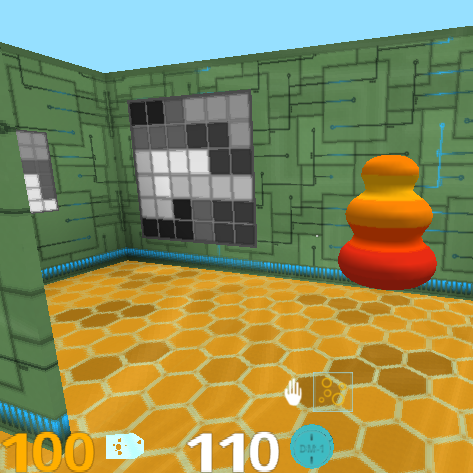
\includegraphics[width=6.61cm,height=6.61cm]{dl-01.png}};
        
        
\pic[shift={(1.8,0,0)}] at (image-east) {RightBandedBox={name=conv1,caption=conv1,%
xlabel={{"32",""}},zlabel=,fill=\ConvColor,bandfill=\ConvReluColor,%
height=28,width={3},depth=28}};

\pic[shift={(1.8,0,0)}] at (conv1-east) {RightBandedBox={name=conv2,caption=conv2,%
xlabel={{"32",""}},zlabel=,fill=\ConvColor,bandfill=\ConvReluColor,%
height=23,width={3},depth=23}};


% shared stream
\pic[shift={(1.8,0,0)}] at (conv2-east) {RightBandedBox={name=conv3,caption=conv3,%
xlabel={{"64",""}},zlabel=,fill=\ConvColor,bandfill=\ConvReluColor,
height=18,width={6},depth=18}};

\pic[shift={(1.1,0,0)}] at (conv3-east) {RightBandedBox={name=conv4,caption=conv4,%
xlabel={{"32",""}},zlabel=,fill=\ConvColor,bandfill=\ConvReluColor,
height=18,width={4},depth=18}};

\pic[shift={(2.6,0,0)}] at (conv4-east) {RightBandedBox={name=fc,caption=fc,%
        xlabel={{"",""}},zlabel=512,fill=\FcColor,bandfill=\FcReluColor,%
        height=3,width=3,depth=50}};

%%%%%%%%%%%%%%%%%%%%%%%%%%%%%%%%%%%%%%%%%%%%%%%%%%%%%%%%%%%%%%%%%%%%%%%%%%%%%%%%%%%%%%%%
%% Draw Arrow Connections
%%%%%%%%%%%%%%%%%%%%%%%%%%%%%%%%%%%%%%%%%%%%%%%%%%%%%%%%%%%%%%%%%%%%%%%%%%%%%%%%%%%%%%%%
\draw [connection]  (image-east)        -- node {\midarrow} (conv1-west);
\draw [connection]  (conv1-east)        -- node {\midarrow} (conv2-west);
\draw [connection]  (conv2-east)        -- node {\midarrow} (conv3-west);
\draw [connection]  (conv4-east)        -- node {\midarrow} (fc-west);
\draw [connection]  (conv3-east)        -- node {\midarrow} (conv4-west);
\draw [connection]  (fc-east)   -- node {\midarrow} ++(1.5,0,0);

\end{tikzpicture}
\end{document}
